\chapter{Multi-machine Implementations}\label{sec-beyond}

In this chapter, we present the integration of Mars into a CPU-based distributed MapReduce system, specifically Hadoop in our implementation. 
This integration benefits from both worlds: Hadoop utilizes CPUs on multiple machines and provides fault-tolerance and other features of a distributed system; 
Mars utilizes the GPU to accelerate local computation. We denote Mars-enabled Hadoop as MarsHadoop. 

We use the {\em Hadoop Streaming}
technology~\footnote{http://hadoop.apache.org/common/docs/r0.15.2/streaming.html}
to integrate Mars into Hadoop. {\em Hadoop Streaming} enables the
developers to use their own custom Map or Reduce implementation in
Hadoop. In our implementation, we use the Mars executable to read
the input from {\em stdin} and to emit the output to {\em stdout}.
Thus, the Map and the Reduce tasks can be performed on the GPU, and
other tasks such as task scheduling and failure handling are
performed by Hadoop. Finally, since current GPUs do not support
multi-tasking, we configure MarsHadoop to run GPU-based tasks sequentially on one GPU. 


Figure \ref{fig:hadoop} illustrates the workflow of MarsHadoop. 
A Map Worker/Reduce Worker in MarsHadoop is the same as a Map Worker/Reduce Worker shown in Figure \ref{fig:Mars+}; 
in other words, it can be from MarsCUDA, MarsBrook, or MarsCPU, depending on the underlying processor. 
In the configuration of Figure \ref{fig:hadoop}, Node 1 simultaneously runs two Map Workers, on a GPU and a CPU respectively. 

\begin{figure}[ht]
  \centering
  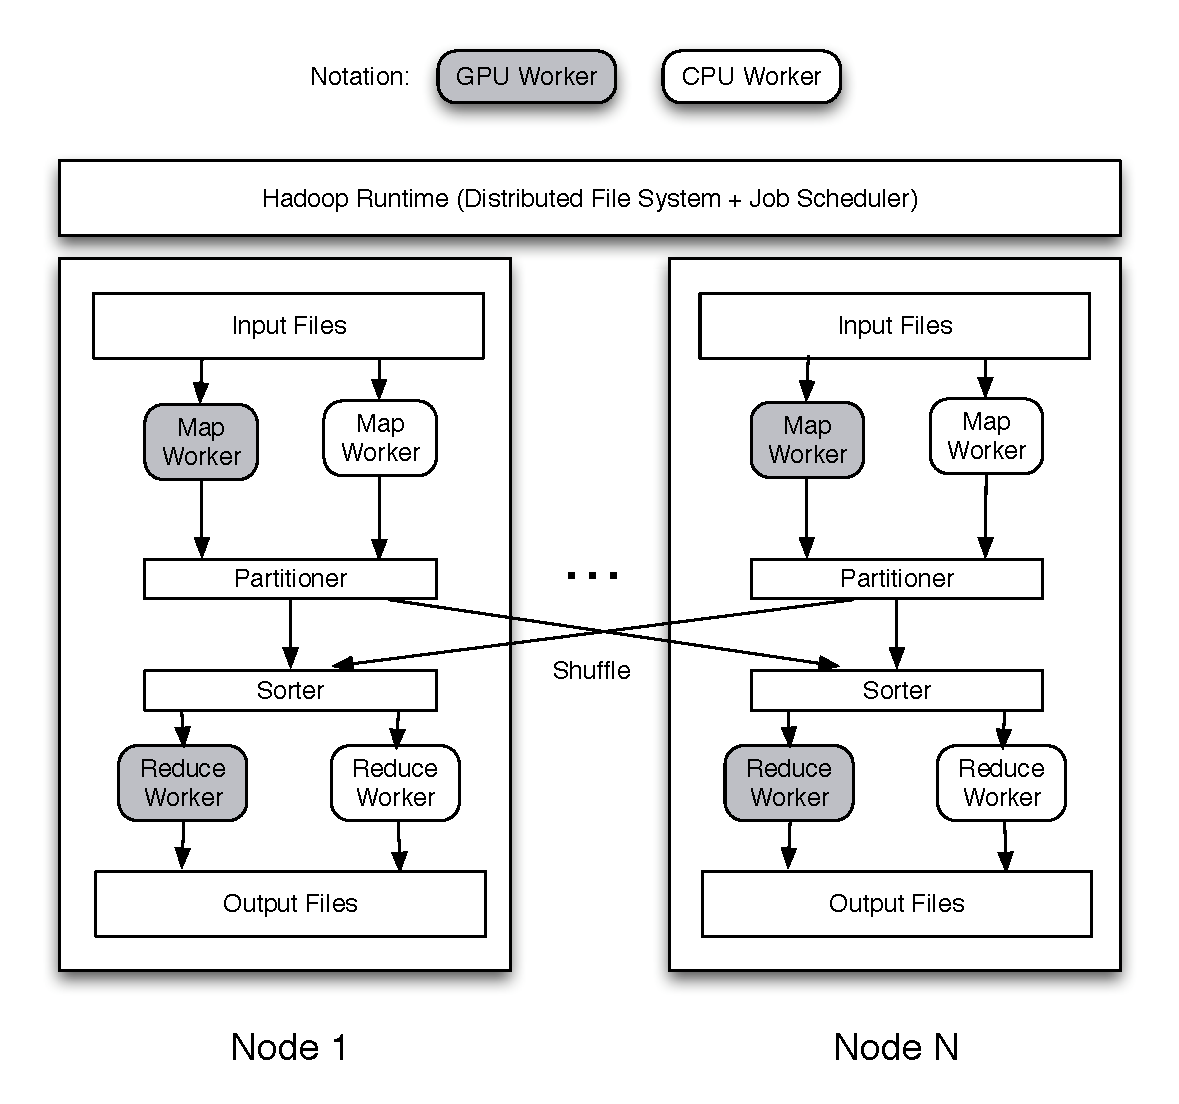
\includegraphics[width=0.70\textwidth]{figure/hadoop.eps} 
  \caption{MarsHadoop. Some Map and Reduce tasks are performed on the
  GPU, and others are on the CPU. }\label{fig:hadoop}
\end{figure}
